A rosa dos ventos � uma figura que representa oito sentidos, que dividem o c�rculo em partes iguais.
\begin{figure}[H]
\centering
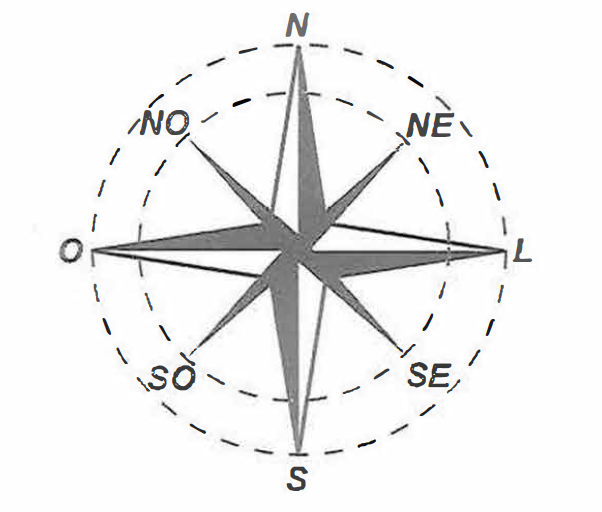
\includegraphics[width=8cm]{../figuras/q140-2018.png}
\end{figure}
Uma c�mera de vigil�ncia est� fixada no teto de um shopping e sua lente pode ser direcionada remotamente, atrav�s de um controlador, para qualquer sentido. A lente da c�mera est� apontada inicialmente no sentido Oeste e o seu controlador efetua tr�s mudan�as consecutivas, a saber: 
\begin{itemize}
\item 12 mudan�a: 135� no sentido anti-hor�rio;
\item 22 mudan�a: 60� no sentido hor�rio;
\item 32 mudan�a: 45� no sentido anti-hor�rio.
\end{itemize}
Ap�s a 32 mudan�a, ele � orientado a reposicionar
a c�mera, com a menor amplitude poss�vel, no sentido Noroeste (NO) devido a um movimento suspeito de um cliente. 
Qual mudan�a de sentido o controlador deve efetuar para reposicionar a c�mera? 
\begin{enumerate}
\item[a)]75� no sentido hor�rio.
\item[b)]105� no sentido anti-hor�rio.
\item[c)]120� no sentido anti-hor�rio.
\item[d)]135� no sentido anti-hor�rio.
\item[e)]165� no sentido hor�rio.
\end{enumerate}
